\chapter{Założenia projektowe}
\label{chap:zalozenia-projektowe}
\section{Wymagania funkcjonalne}
\label{sec:wymagania-funkcjonalne}

W tej sekcji opisane zostaną wymagania funkcjonalne jakie powinien spełniać stworzony system. Zaprezentowane zostaną przypadki użycia dla czterech podsystemów: system zarządzania kontem pieniężnym, system zarządzania środkami finansowymi, system zarządzania rodziną i system zarządzania kategoriami. Przypadki użycia zostaną opisane w schemacie: nazwa przypadku użycia, aktor wykonujący akcję, warunki początkowe, warunki końcowe, cel oraz przebieg. Ponadto przypadki użycia zostaną zaprezentowane w formie diagramów.

\subsection{Wymagania dotyczące konta pieniężnego}
\label{subsec:wymagania-konto}
Poniżej opisano przypadki użycia dotyczące zarządzania kontem pieniężnym użytkownika. Zaprezentowano je także na diagramie (rys.~\ref{fig:use-case-account}).

\begin{enumerate}[labelwidth=1em,label=\arabic*.]
\item \textbf{Nazwa:} Dodaj konto \newline
    \textbf{Aktor:} Zalogowany użytkownik \newline
    \textbf{Warunki początkowe:} Użytkownik musi posiadać wcześniej założone konto i się na nie zalogować. \newline
    \textbf{Warunki końcowe:} Stan konta musi być zgodny z polityką dla jego typu. \newline
    \textbf{Cel:} Stworzenie w systemie konta pieniężnego przypisanego do aktora wykonującego tę operację, aby umożliwić zapisywanie informacji o przepływie gotówki. \newline
    \textbf{Przebieg:} Użytkownik wypełnia formularz. Wpisuje wymagane pola: nazwa konta, saldo początkowe i limit debetu oraz opcjonalne pola: numer konta, waluta i opis. Wybiera także typ konta.
\item \textbf{Nazwa:} Usuń konto \newline
    \textbf{Aktor:} Właściciel konta \newline
    \textbf{Warunki początkowe:} Użytkownik musi posiadać konto pieniężne. \newline
    \textbf{Warunki końcowe:} Użytkownik musi potwierdzić usunięcie konta. \newline
    \textbf{Cel:} Usunięcie konta pieniężnego użytkownika wraz z jego historią. \newline
    \textbf{Przebieg:} Użytkownik wybiera jedno ze swoich kont, a następnie naciska guzik usuń. Użytkownik musi potwierdzić tę operację.
\item \textbf{Nazwa:} Edytuj dane konta \newline
    \textbf{Aktor:} Właściciel konta \newline
    \textbf{Warunki początkowe:} Użytkownik musi posiadać konto pieniężne. \newline
    \textbf{Warunki końcowe:} Stan konta nie może przekraczać nowego limitu debetu. \newline
    \textbf{Cel:} Aktualizacja danych konta, bez utraty jego historii. \newline
    \textbf{Przebieg:} Użytkownik edytuje pola obowiązkowe formularza: nazwa konta, limit debetu oraz opcjonalne pola: numer konta, waluta i opis. Nie może edytować jego typu.
\item \label{last-item1}\textbf{Nazwa:} Zmień typ konta\newline
    \textbf{Aktor:} Właściciel konta \newline
    \textbf{Warunki początkowe:} Użytkownik musi posiadać konto pieniężne. \newline
    \textbf{Warunki końcowe:} Typ konta musi pozwalać na potencjalnie istniejący na koncie debet. \newline
    \textbf{Cel:} Zmiana typu konta na inny. Umożliwiające posiadanie debetu, lub oprocentowane. \newline
    \textbf{Przebieg:} Użytkownik po wybraniu konta zmienia jego typ, a swój wybór zatwierdza naciśnięciem guzika ,,Akceptuj''. 
\end{enumerate}

\begin{figure}[t]
	\centering
	\fbox{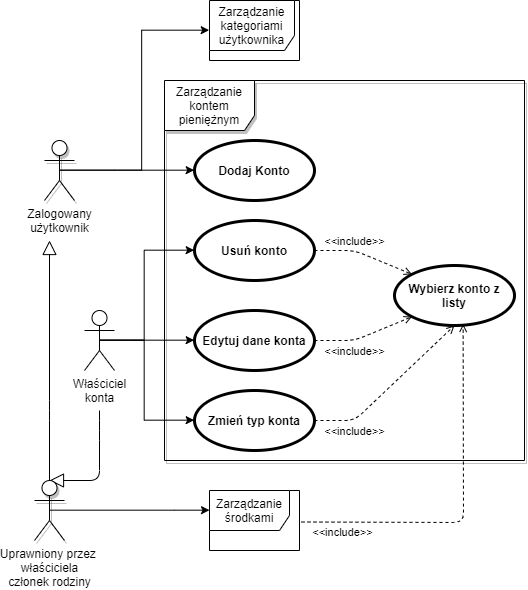
\includegraphics[width=.65\linewidth]{rys03/use-case-account.png}}
	\caption{Diagram przypadków użycia konta pieniężnego}
	\label{fig:use-case-account}
\end{figure}

\subsection{Wymagania dotyczące środków finansowych}
\label{subsec:wymagania-srodki-finansowe}
Na rysunku~\ref{fig:use-case-money} przedstawiono przypadki użycia związane z definiowaniem przepływu gotówki w ramach kont pieniężnych. Poniżej znajdują się także ich opisy.

\begin{enumerate}[labelwidth=1em,label=\arabic*.]
\item \textbf{Nazwa:} Dodaj wydatek/przychód \newline
    \textbf{Aktor:} Właściciel konta \newline
    \textbf{Warunki początkowe:} Użytkownik zdefiniował co najmniej jedną kategorię dla operacji finansowych. \newline
    \textbf{Warunki końcowe:} Stan konta po operacji dodania wydatku musi być zgodny z polityką dla typu konta. \newline
    \textbf{Cel:} Zdefiniowanie operacji pieniężnej w ramach konta. \newline
    \textbf{Przebieg:} Użytkownik tworzy wydatek lub przychód wpisując obowiązkowe pola: kwota i data, a także te dodatkowe: notatka, odbiorca. Użytkownik musi także wybrać kategorię. 
\item \textbf{Nazwa:} Usuń wydatek/przychód \newline
    \textbf{Aktor:} Właściciel konta \newline
    \textbf{Warunki początkowe:} Konto posiada co najmniej jeden wpis: wydatek lub przychód. \newline
    \textbf{Warunki końcowe:} Stan konta po operacji usunięcia przychodu musi być zgodny z polityką dla typu konta. \newline
    \textbf{Cel:} Usunięcie operacji pieniężnej w ramach konta. \newline
    \textbf{Przebieg:} Użytkownik wybiera wydatek lub przychód, a następnie naciska guzik usuń. 
\item \textbf{Nazwa:} Edytuj wydatek/przychód \newline
    \textbf{Aktor:} Właściciel konta \newline
    \textbf{Warunki początkowe:} Konto posiada co najmniej jeden wpis: wydatek lub przychód. \newline
    \textbf{Warunki końcowe:} Stan konta po edycji wpisu musi być zgodny z polityką dla typu konta. \newline
    \textbf{Cel:} Edycja operacji pieniężnej w ramach konta. \newline
    \textbf{Przebieg:} Użytkownik wybiera wydatek lub przychód, a następnie naciska guzik ,,edytuj''. Edytuje pola obowiązkowe i dodatkowe. Jeśli chce zmienić kategorię musi ją wybrać z listy. \newline
    \textbf{Rozszerzenia: } 
    \begin{enumerate}[label=\alph*)]
        \item Użytkownik edytuje kategorię wpisu: Wybór kategorii.
    \end{enumerate}
\item \textbf{Nazwa:} Wykonaj przelew \newline
    \textbf{Aktor:} Właściciel konta \newline
    \textbf{Warunki początkowe:} Użytkownik zdefiniował co najmniej jedną kategorię dla operacji finansowych. \newline
    \textbf{Warunki końcowe:} Stan konta po przelewie musi być zgodny z polityką dla typu konta. \newline
    \textbf{Cel:} Wykonanie przelewu między kontami \newline
    \textbf{Przebieg:} Użytkownik definiuje przelew wpisując obowiązkowe pola: kwota i data, a także dodatkowe: notatka, odbiorca. Użytkownik musi także wybrać kategorię. \newline
    \textbf{Rozszerzenia: } %TODO strzalka icnlude do wybierz kategorie
    \begin{enumerate}[label=\alph*)]
        \item Użytkownik definiuje przelew między własnymi kontami: Przelew własny.
    \end{enumerate}
\end{enumerate}

\begin{figure}[t]
	\centering
	\fbox{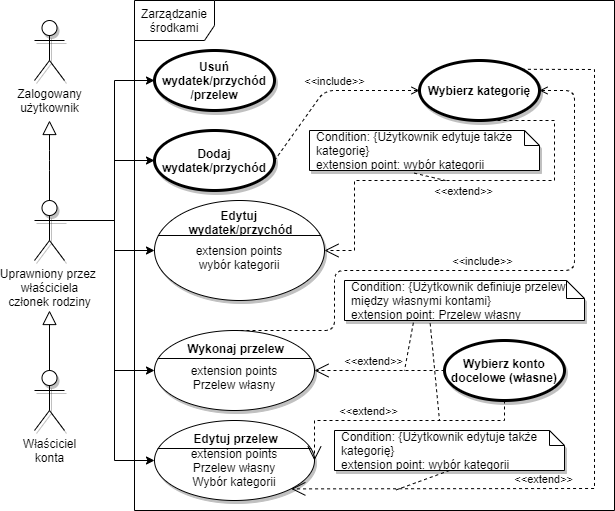
\includegraphics[width=.7\linewidth]{rys03/use-case-money.png}}
	\caption{Subdiagram przypadków użycia dla operacji finansowych}
	\label{fig:use-case-money}
\end{figure}

%Na razie do wglądu diagramy use cases
% Jest kilka kwestii do dyskusji
% W systemie powinny być kategorie usera i rodziny. User moze edytowac swoje kategorie a admin rodziny rodzinne kategorie. Gdy konto jest dodane do rodziny mozna mu dodawac kategorie rodziny ale tez usera
% 1 pytanie czy use case diagram dla category jest poprawny (generalizacja) Moze powinny byc osobne use casy dla kategorii rodziny i osobne dla kategorii usera

%2 family use case: czy admin powinien moc nadawac uprawnienia do nieswojego konta? Cz powinien admin moze domyslnie i zawsze dodawac wydatki do nieswojego konta, czy moze wlasciciel musi mu nadac uprawninia. 

\begin{figure}[p]
	\centering
	\fbox{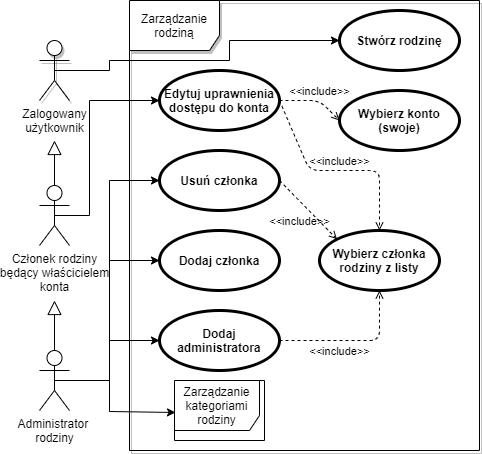
\includegraphics[width=.65\linewidth]{rys03/use-case-family.png}}
	\caption{Diagram przypadków użycia dla kategorii}
	\label{fig:use-case-category}
\end{figure}

\begin{figure}[p]
	\centering
	\fbox{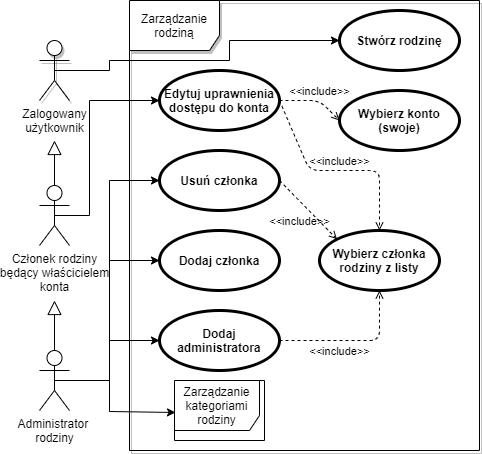
\includegraphics[width=.65\linewidth]{rys03/use-case-family.png}}
	\caption{Diagram przypadków użycia dla rodziny}
	\label{fig:use-case-family}
\end{figure}


\section{Wymagania niefunkcjonalne}
\label{sec:wymagania-niefunkcjonalne}

\begin{enumerate}[labelwidth=1em,label=\arabic*.]

\item System składać ma się z~dwóch głównych części:
\begin{enumerate}[label=\alph*)]
\item aplikacji serwerowej -- API. Jej zadaniem będzie dostarczanie interfejsu programistycznego do pobierania danych i~modyfikowania stanu systemu.
\item aplikacja webowej, dostarczająca graficzny interfejs użytkownika -- \texttt{GUI}. Aplikacja ta będzie konsumować API.
\end{enumerate}

\item Zarówno aplikacja webowa, jak i API będą stworzone przy pomocy frameworka ASP.NET Core w wersji co najmniej 2.2: 
\begin{enumerate}[label=\alph*)]
\item Do napisania aplikacji webowej użyte zostaną \texttt{Razor Pages} oraz komponenty widoku (ang.~\emph{view components}). 
\item Warstwa persystencji danych w aplikacji API stworzona zostanie z pomocą Entity Framework Core 2.2. Wykorzystane zostanie podejście \emph{code first} i mechanizm migracji.
\end{enumerate}

\item Pobieranie danych z API ma odbywać się za pomocą protokołu OData.

\item API używać będzie bazy danych na serwerze Microsoft SQL Server 2017 (lub nowszym).

\item Aplikacja webowa powinna poprawnie działać co najmniej w przeglądarkach: Mozilla Firefox, Google Chrome, Opera, Microsoft Edge oraz Safari, a~także przeglądarkach mobilnych: Opera Mobile, Google Chrome, Mozilla Firefox i Safari.

\item Aplikacja będzie wymuszać działanie z wykorzystaniem protokołu \texttt{HTTPS} (ang.~\emph{Hypertext Transfer Protocol Secure}).

\item Autoryzacja i uwierzytelnienie ma być przeprowadzona z wykorzystaniem protokołu OpenId Connect i frameworka autoryzacji OAuth 2.0. Użyty powinien zostać \emph{Hybrid Flow} lub \emph{Authorization Code Flow}.

\item Dostawcą tożsamości w systemie powinna być osobna aplikacja, posiadająca własną bazę danych lub zewnętrzy system autoryzacji, np.~\texttt{Auth0}.

\item API ma posiadać dokumentację stworzoną przy pomocy narzędzia \texttt{Swagger}.

\item Kod źródłowy ma być napisany z wykorzystaniem dobrych praktyk programowania~i~wzorców projektowych ułatwiających jego utrzymanie i rozwijanie.

\item System działać będzie na platformie chmurowej \texttt{Microsfot Azure}.

\item Poszczególne składowe systemu w chmurze powinny być automatycznie skalowalne.

\item Aplikacja webowa powinna być bezpieczna i odporna na ataki. Zostanie wykorzystany mechanizm obrony przed \texttt{CSRF} (ang.~Cross-Site Request Forgery) -- \texttt{anti-forgery token}.

\end{enumerate}

\section{Metodyka}
\label{sec:metodyka}